% !TEX root = ../thesis-example.tex
%
\chapter{Introduction}
\label{ch:introduction}
%
%\cleanchapterquote{L'instrument est un compromis instable\\entre des qualités non-convergentes.}{Bernard Sève}{(L'instrument de musique: une étude philosophique \cite{seve_instrument_2013})}

\cleanchapterquote{MUSIQUE. \textit{Petit orchestre en train de s'accorder doucement.}\\
PAROLES. —~Pitié! (\textit{Orchestre. Plus fort.}) Pitié! (\textit{L'orchestre faiblit, se tait.}) Combien de temps encore à moisir ici dans le noir ? (Avec dégoût.) Avec toi! (\textit{Un temps.})}
{Samuel Beckett}{\textit{paroles et musique}. 1962.}

\vspace*{\fill}

%\Pierre{ l'introduction doit présenter le titre : représentation, contrôle, desgin interactif, instrument de musique et instrument de musique numérique (pas forçément dans cet ordre)}

%\Pierre{ je pense que tu devrais ici repartir du début : tes motivations pour ce sujet et quels sont les notions que tu dois absolument présenter pour que l'on comprenne ta problématique. Typiquement, une intro de thèse = contexte -> problématique/hypothèses -> annonce du plan}
\noindent {\Large \textbf{Rewind~/~Record~/~Fast-Forward}}

\noindent J'ai commencé l'étude d'un ``vrai'' instrument de musique --~le saxophone~-- en école de musique à l'âge de 12 ans, mais n'ai réalisé que des années plus tard que le premier instrument de musique que j'avais pratiqué avait six touches et deux contrôleurs continus: REC, PLAY, PAUSE, STOP, RWD, FWD, un contrôle de volume et un sélecteur de fréquence radio. Né au moment de l'invention du Walkman™ et de la ``libération des ondes'', j'ai rapidement eu entre les mains cet objet que peu auraient appelé ``instrument de musique'' à cette époque (sauf  dans des endroits comme le \gls{GRM} mais ils m'étaient inconnus à cet âge), qui permettaient pourtant de jouer des sons, des sons venant d'ailleurs ou des sons personnels, enregistrés ``à la main''. Le balladeur, comme son nom l'indique en français ou en anglais, permettait d'emmener son instrument partout, à la condition d'avoir des piles chargées, en classe comme le long des trajets de bus ou de voiture, et a probablement constitué la pratique musicale principale de toute ma génération en nombres d'heures passées sur son instrument.
\begin{wrapfigure}[4]{r}{0.25\textwidth}
	\vspace{-6.2em}
	\captionsetup{format=plain}
	\centering
 	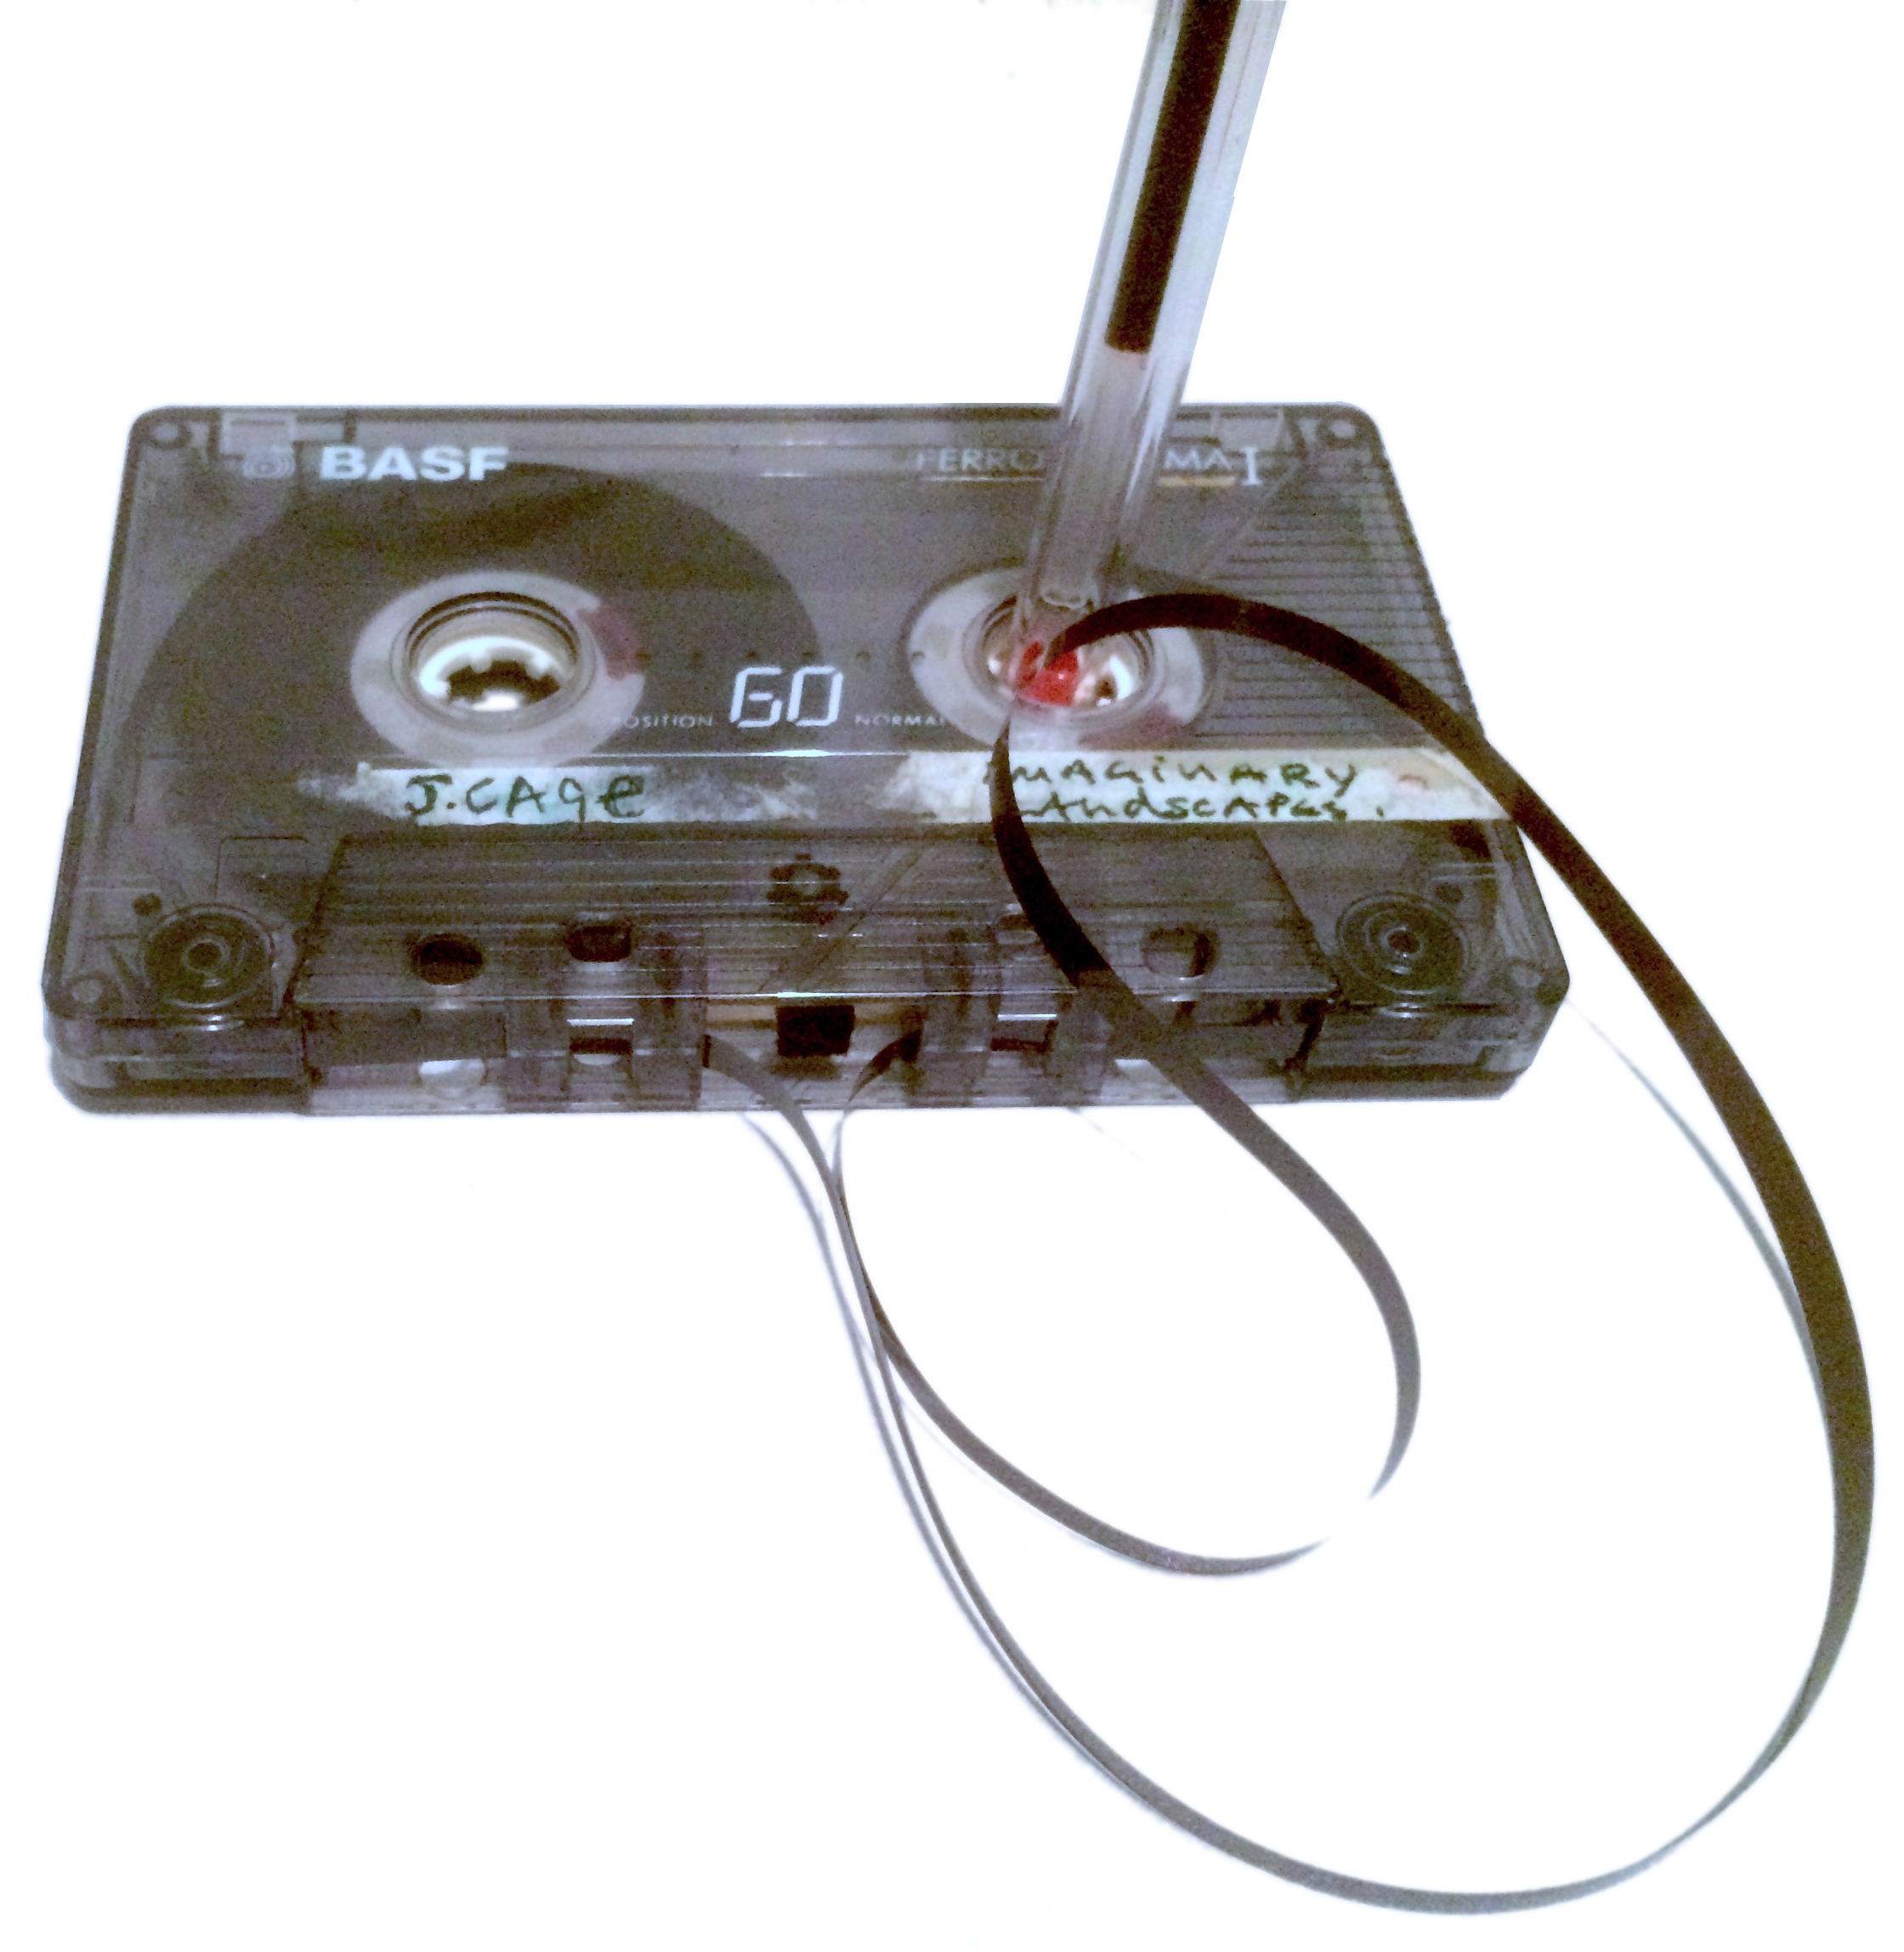
\includegraphics[width=0.56\textwidth]{gfx/01_preamble/K7.png}
 	%\vspace{-2em}
	%\caption[Walkman.]{Walkman.}
 	\label{fig:preamble:walkman}
\end{wrapfigure}
\par
\indent Aurais-je été en droit d'appeler mon balladeur-enregistreur un ``instrument'' ? Il n'existait aucun répertoire, aucune partition, aucun professeur enseignant sa pratique et en premier lieu, aucun musicien jouant d'un tel instrument en concert. Pourtant il y avait un public et je n'étais pas le seul auditeur; l'échange entre amis de compilations sur cassettes audio nous permettait de partager des morceaux, et à défaut d'en être les auteurs, nous étions les auteurs de nos sélections musicales.\\
\indent Une dizaine d'années plus tard, la dédicace que je lis à l'ouverture de l'imposant \textit{Traité des objets musicaux} de Pierre Schaeffer se fait l'écho : \iquote{À la mémoire de mon père, violoniste, dont je transmets le précepte : Travaille ton instrument}. 
Ce précepte qui prend la forme d'une injonction laisse imaginer la scène du père qui ordonne au petit Pierre d'aller faire ses gammes. Mais quel est donc l'instrument que Pierre Schaeffer semble avoir suffisamment travaillé pour reprendre ce précepte en ouverture de son ouvrage majeur ? Le disque à sillon fermé ? Le \textit{Phonogène} ? Où s'agirait-il davantage de sa propre perception auditive, dont il entreprend l'étude systématique pour en déchiffrer les ``modes de jeu'' ?

\indent Ce travail de recherche a commencé après plus de 15 années passées à concevoir, fabriquer, programmer, pratiquer et écouter des instruments de musique à l'aide d'ordinateurs. J'ai créé durant ces années diverses sortes d'applications, d'instruments, d'installations, d'outils, dans différents contextes : spectacle vivant, installations multimédia, ateliers pédagogiques, expositions muséographiques, émissions de radio, projets de recherche, etc. Il est sûrement vain de vouloir discriminer parmi tous ces objets lesquels constituent des instruments de musique et lesquels n'en sont pas, mais il me semble intéressant de constater que ces développements posent à chaque fois, sous différents angles, la question du rapport de musicalité avec la machine. C'est ce constat qui m'a amené à réfléchir sur ma pratique et sur la notion d'instrument de musique numérique pour essayer d'en cerner les contours, ou du moins, d'en percevoir les lignes de fuite.

\indent Poser la question de sa représentation, face à un medium numérique qui fait voler l’objet en éclat ainsi que les traditions musicales qu’il sous-tend, pose imanquablement celle des motivations pour lesquelles nous construisons des instruments, et par suite, des raisons pour lesquelles nous inventons, pratiquons, écoutons la musique. De cela découlent les multiples manières dont nous jouons avec le réel, avec les objets, avec les sons pour produire cet étrange --~et pourtant si familière~-- vibration de l'air.\\
\indent La notion d’instrument de musique numérique embrasse ces problématiques, complexes sur le plan technique, mais davantage encore sur le plan sociologique et esthétique. La façon dont nous créons la musique et la manière dont nous l’écoutons a tellement changé en un siècle qu’il semble désuet de tenter de l’aborder sur un plan purement technique, tant celle-ci semble promise à bouleverser encore davantage nos usages dans l’avenir. Le travail présenté dans cette thèse n'entend pas répondre à ces questions bien trop vastes mais tâchera, autant que possible, de ne pas perdre de vue les raisons profondes du désir musical, souvent difficile à expliquer et ranger dans des catégories et des articulations logiques.


\section{Une thèse interdisciplinaire}

sciences exactes + sciences humaines + pratique musicale

\noindent Cette thèse a été l'objet d'un contrat doctoral soutenu par le Collegium Musicæ, dont la mission est de promouvoir l'interdisciplinarité entre différents acteurs institutionnels œuvrant dans le champ de la musique. En l'occurence, cette thèse a été co-dirigée par Pierre Couprie, musicologue à l'\gls{IReMus} et Jean-Dominique Polack et Hugues Genevois, chercheurs de l'équipe \gls{LAM}. En se situant entre les domaines distincts des sciences et de l'ingénierie d'une part et de la musicologie d'autre part, cette thèse est la tentative d'une étude des \glspl{DMI} prenant ces deux dimensions en compte.

Par ailleurs, ce travail de recherche théorique est soutenu par des développements techniques disponibles librement sur Internet et dont j'espère qu'ils pourront profiter à la communauté des musiciens intéressés par ces outils.
Enfin, elle s'appuie sur des performances musicale mettant en œuvre ces développements pour confronter la théorie à la pratique tout autant que pour affiner la théorie sur la base de l'observation de ces pratiques. Elle constitue donc un travail de une recherche à la fois basée sur la pratique et dirigée par la pratique.


ajouer (éventuellement?) un mot sur les usages, formats et conférences relativement différentes et séparées dans ces domaines. 
Evolution vers une interdisciplinarité nécessaire à la compréhension mutuelle. Cf. présence d'article musicologie dans NIME.


\section{Qu'entend-on par ...}

\noindent Il s'agit ici de donner quelques éléments permettant de préciser la signification donnée à un certain nombre de termes dans ce document.

\subsection*{``Représentation...}

\noindent Le terme ``représentation'' recouvre un très vaste champ sémantique. Si son étymologie évoque le fait de ``rendre de nouveau présent'', la représentation passe aussi par l'image --~réelle ou mentale~--, distincte de l'originale représenté, que l'on se fait de quelque chose.

La question de la réprésentation (ou plutôt, des représentations) dans les lutheries numériques est envisagée sous différents angles, et présente ainsi des significations variables dans ce document : 
\vspace{-1em}
\begin{itemize}[noitemsep]
\item la représentation organologique des \glspl{DMI}, en particulier les manières variées dont il se présente comme agencements modulaires (ch. \ref{ch:ephemeral}) en contraste avec les représentations plus monolithiques de l'instrument classique;
\item la représentation de ce que l'on appelle communément ``le geste musical'' du point de vue des \glspl{DMI}(ch. \ref{ch:gesture});
\item la représentation physique du \gls{DMI} en tant qu'interface entre la continuité analogique du monde physique et l'espace discret de son inscription algorithmique, en particulier son aspect visuel dynamique lié à l'usage de l'infographie (ch. \ref{ch:interfaces});
\item la représentation proposée par le langage informatique dans lequel s'exprime le design de l'interaction musicale dans les \gls{DMI}, en particulier la manière dont s'articulent les messages venant représenter les données (gestuelles, audio, visuelles, etc.) à l'œuvre dans un \gls{DMI}, sous forme de signaux continus ou d'événements discrets (ch. \ref{ch:algorithms});
\item la représentation visuelle de l'interface de jeu, et en particulier son aspect dynamique lié à l'usage de l'infographie (ch. \ref{ch:visual_representation});
\item la représentation des éléments de vocabulaire musical dans le cas de l'improvisation électroacoustique jouée avec ces instruments numériques, en vue de leur notation (ch. \ref{ch:notation}).
\end{itemize}

\subsection*{...et contrôle...}

\noindent Le contrôle est éminemment lié à la question de la représentation, ce couple formant deux versants complémentaires --~action et perception~-- du phénomènes d'interaction. En l'occurence, si dans le cas des instruments acoustiques, on agit sur l'instrument dans le but de contrôler le son qu'il produit, on agit dans le cas des \gls{DMI} sur des représentations de sons et de gestes encodé sous la forme de données numériques. La question du geste instrumental y tient une place centrale et nous verrons notamment comment la causalité entre gestes et sons, se ré-articule dans le cas des \glspl{DMI}.

\subsection*{...dans le design interactif...}

\noindent Ces aspects de représentation et de contrôle sont ici étudiés dans la perspective concrète de leur prise en compte dans le travail de lutherie numérique. Le terme ``design interactif'' est un emprunt à l'anglais \iquote{interactive design}, généralement traduit par ``design de l'interaction'', c'est-à-dire la conception et la réalisation des fonctions qui assurent l'aspect interactif de l'objet que l'on conçoit. Cependant, sa version anglaise laisse entendre l'aspect interactif du processus de design lui même, ce qui reflète dans une grande mesure la manière dont le développement d'un \gls{DMI} (et des instruments de musique, de manière plus générale) se passe : dans un jeu permanent d'aller-retours entre la fabrication, la programmation, la pratique et l'écoute.

\subsection*{...des instruments...}

\noindent Une définition simple et efficace des instruments de musique serait la suivante : ``tout dispositif dont on se sert pour musiquer''. Cette définition qui peut apparaître comme un truisme présente l'intérêt de ne pas définir les instruments en fonction de leur nature ou de leur caractéristiques techniques, mais en fonction de leur usage. En particulier, l'utilisation du terme ``jouer'' vient préciser que, si de nombreux objets techniques permettent depuis le \siecle{20}siècle de ``produire'' de la musique à partir d'enregistrement, il ne sont envisageables en tant qu'\textit{instruments de musique} que s'ils sont joués, et non simplement ``utilisés''. Ainsi, la platine vinyle est un instrument de reproduction sonore quand elle est utilisée par le mélomane dans son salon, mais le même objet sera un instrument de musique s'il est joué.

On pourrait alors poser la question des contours que recouvrent le terme jouer.
Les instruments de musique ne sauraient donc être définis qu'à l'aune de la définition que l'on veut bien donner au terme musique. Une perspective intéressante du terme ``instrument'' cependant est sa double polarité d'objet qui sert à la fois à agir sur le monde (l'instrument-outil) et à le sentir (l'instrument de mesure).
Etymologie : \textit{struo} = construire, disposer, empiler, tramer.  \textit{instruo} : instruire, enseigner, former.

\iquote{Musiquer, c'est prendre part, quelqu'en soit notre capacité, à une performance musicale. Cela signifie non seulement jouer, mais aussi écouter, fournir des matériaux pour la performance --~ce que nous appelons composer~--, se préparer pour une performance --~ce que nous appelons répéter ou pratiquer~-- et tout autre activité connectée à la performance musicale. Nous devons certainement inclure le fait de danser, si quelqu'un danse, et nous pourrions même étendre la signification à l'occasion pour inclure ce que fait la dame qui prend les tickets à l'entrée, les gros bras qui déplacent le piano, ou les roadies qui préparent les instruments et portent le matériel de son, étant donné que leurs activités affectent également la nature de l'événement qu'est une performance musicale.}
\cite{small_musicking:_1998}

\Pierre{21-08 C'est super de parler de Small mais attention, tu mets un pied dans la sociologie et c'est bien dans ce périmètre qu'il conçoit le ‘musicking’. Je ne pense pas que cela corresponde à ce que tu nommes précédemment ‘musiquer’, ‘musicking’ est bien plus large.}

The digital has engendered a sense of novelty, curiosity, and originality in terms of performance, sound and music. The musical \textit{results} are strongly dependant on the instrument, and they often \textit{are} the instruments. Magnusson, Sonic Writing, p.61

Les instruments de musique sont des instrument pour jouer de la musique (ou pour musiquer, dirait Christopher Small \cite{small_musicking:_1998}). Cette apparente évidence est nécessaire pour signaler qu'il ne s'agit pas simplement de faire des notes, ou même du son. La musique implique également notre \textit{mémoire du son}, l'imagination que nous en avons, les aspects visuels qui se rattachent à la notion de musicalité, et d'autres dimensions esthétiques et culturelles. \todo{être plus précis}

La performance musicale a cela de particulier qu'elle ne possède pas de cahier des charges préalables (la partition ne saurait être considérée comme telle!) et que loin de se plier à la nécessité d'exécuter une tâche précise, comme il pourrait être le cas dans le design d'autres interfaces homme-machine, les instruments sont des objets techniques dont les musiciens abusent (plus qu'ils en usent), dont les artefacts peuvent être appréciables et souhaitables, dont la compréhension n'est pas un préalable requis pour leur utilisation, pas davantage que leur fiabilité n'est garante d'une performance musicale intéressante.

\Pierre{21-08 Ce paragraphe est une excellente definition de l'instrument numérique. C'est vraiment très bien dit.}

%
Le design des \glspl{DMI}, ainsi que le design des outils-mêmes du luthier numérique, doivent être informés de ces particularités propres à la création artistique si l'on souhaite qu'ils se prêtent à la création de musiques nouvelles et à l'exploration de territoires sonores inexplorés.


\subsection*{...de musique...} 
\subsubsection*{définition intrinsèque}
La musique est un concept difficile à définir et comme le dit le musicologue Pierre Billard en intoduction de la définition donnée par l'encyclopédie Universalis \iquote{plus notre connaissance de la musique est étendue et moins nous savons, en fin de compte, ce qu'elle est.}

Définir la musique sur la base de son contenu est probablement la perspective la moins consensuelle qui soit et dont l'intérêt principal est peut-être qu'elle qualifie surtout l'opinion de celui (ou du groupe) qui la définit ainsi : musique de son purs, musique de bruits, sons organisés de Varèse.
\subsubsection*{définition intrinsèque}

On peut définir la musique du point de vue de celui qui la produit (compositeur, instrumentiste) : « Tout corps sonore utilisé par le compositeur est un instrument de musique. » Berlioz, 1843, Grand Traité d'instrumentation et d'orchestration modernes

Définir la musique du point de vue de celui qui l'écoute : est musique tout ce que j'écoute et considère comme telle.

La musique est un art de la résonance, qu'elle soit d'ordre acoustique et physique, ou d'ordre plus intellectuelle et spirituelle. La musique fait écho.

\subsection*{...numériques}

\indent On parle souvent, par métonymie, des ``musiques électroniques'' ou ``musiques numériques'' pour désigner des productions musicales où l'empreinte de ces medias caractérise de manière prononcée une certaine esthétique. Mais le terme ``numériques'', dans le titre de cette thèse, est au pluriel car c'est bien le caractère numérique des instruments auquel je m'intéresse dans ce travail et ses conséquences en terme de lutherie. Ces specificités seront analysées plus en détail dans la perspective propre à chaque chapitres, mais j'en évoquerai ici les traits principaux :
\vspace{-1em}
\begin{itemize}[noitemsep]
\item \textbf{le découplage énergétique} : introduit par l'utilisation de l'électricité;
\item \textbf{le représentation symbolique} : qui permet de manière générale l'enregistrement et l'agencement sur un medium commun de données aussi diverses que des échantillons sonores, des algorithmes ou des structures de représentation de données;
\item \textbf{les capacités de stockage en mémoire} : qui permettent notamment le temps différé (davantage que le ``temps réel'') et l'élaboration d'écritures dynamiques 
\item \textbf{la computation} : le traitement algorithmique qui permet --~ou impose~-- une reconfiguration permanente des modèles et des représentations;
\item \textbf{le réseau} l'inscription des \glspl{DMI} dans l'écosystème du numérique, qui permet la distribution, l'échange, la mise en commun, la duplication des ressources sur des modules et plateformes en réseau.
\end{itemize}

J'utiliserai parfois le terme de ``musicien numérique'' au sens où le définit Andrew Hugill comme \iquote{quelqu'un qui a saisi les possibilités ouvertes par les nouvelles technologies, en particulier le potentiel de l'ordinateur pour explorer, stocker, manipuler et traiter le son, ainsi que le développement de nombreux autres outils et dispositifs numériques qui permettent l'invention et la découverte musicale}\footnote{Dans son ouvrage \textit{The Digital Musician} \cite{hugill_digital_2019}}.

C'est ici ce qu'amène le numérique qui m'intéresse, c'est-à-dire ( TODO) l'utilisation d'une forme symbolique automatisée et traitable en grande quantité par les ordinateurs. Ce que cela apporte aux instruments, ce qui unit ou sépare les différents types d'instruments numériques ensemble et par rapport aux lutheries classiques.


\section{Problématique}

\noindent La conception des \glspl{DMI} rassemble des questions qui étaient relativement dissociées dans la lutherie acoustique traditionnelle : les rôles du facteur d'instrument, du compositeur, de l'interprète et de l'auditeur y sont généralement assumés par des personnes distinctes. Les nouvelles lutheries, et particulièrement celles usant de technologies numériques, redistribuent ces fonctions qui bien souvent se retrouvent endossées par une même personne. En particulier, la possibilité de modéliser les savoirs-faire propres à ces différents domaines dans des outils qui prennent en charge tout ou partie de leur mise en œuvre permet de nuancer la part d'implication du \textit{musicien numérique} dans chacun de ces domaines d'expertise.

\indent La question centrale de cette thèse sera donc formulée ainsi : comment, dans cette redéfinition généralisée des interactions entre le geste et le son, le réel et le virtuel, l'écriture et l'interprétation, s'articule l'agencement d'un \gls{DMI} ?

le musicien, son instrument, face auquels s'ouvre un infini des possibles sonores, s'articulent l'agencement d'un \gls{DMI} et l'agentivité relative ?

\Pierre{ Je ne vois pas de problématique présentée. La problématique est la question que tu poses dans ta thèse ainsi que les questions annexes ou sous-questions.}

Nécessité de prendre en compte la part expérientielle de la performance musicale, notamment dans sa dimension subversive.

Cette thèse propose une étude de la création et la performance musicale avec des \gls{DMI}, pour essayer d'en re-définir les contours et en tirer des conséquences sur leur design.

Notamment, en envisageant le geste musical comme phénomène dépassant l'approche fonctionnelle qui lui est souvent conférée dans les études en \gls{IHM}, et en analysant les \glspl{DMI} en tant qu'assemblages et processus possédant des qualités propres et différentes de celles des instruments acoustiques, ce travail vise à étudier comment les différents enjeux qui se posent avec de tels instruments dans la performance musicale s'articulent au niveau de leur conception.

Quelques questions : 
\vspace{-1em}
\begin{itemize}[noitemsep]
\item Au delà des métaphores de la bureautique (menus, sliders, checkbox), quel vocabulaire graphique est envisageable pour le design des éléments d'interaction ?
\item Comment gérer les scénarios de déconnexion / reconnexion dynamiques intervenant dans le cours d'une performance ?
\item Comment noter la musique (électroacoustique) produite avec de telles interfaces pour le jeu collectif ?
\item Quelles interfaces seront pertinentes lors des différentes phases de conception, de composition, de répétition, ou de performance avec l'instrument ?
\item  Quelles représentations privilégieront, pour le contrôle de paramètres identiques, tantôt la virtuosité, la précision, l'étendue de de la palette sonore, la polyphonie gestuelle ou encore la structure temporelle ?
\end{itemize}

\section{Enjeux et hypothèses}

Enjeu de trouver des caractéristiques transversales dans les lutheries numériques malgré l'absence de tradition, de répertoire, de notation, de méthode d'apprentissage, etc.
Enjeu de confronter au réel des réalisations instrumentales et logicielles à travers une pratique musicale.

Ce travail tente de présenter l'ensemble d'une démarche de création d'un \gls{DMI}, comprenant sa conception, sa fabrication, sa programmation, sa pratique, et la composition avec cet instrument.
Ce travail de recherche s'offre donc comme une présentation ``en coupe'' d'un travail de lutherie, dans ce qu'il comporte de réflexions, de choix de matériaux, d'assemblages, de programmation, de notations, de pratiques et comment ces différents aspects interfèrent dans le cas particulier des instruments intégrant le numérique dans le design de leur interaction.

\subsubsection*{Hypothèse 1 : l'instrument atomisé, recomposé}

L'instrument est atomisé et se retrouve configuré comme un agencement modulaire évolutif qui se cristallise ponctuellement dans des instances contextuelles. \\
Pas d'instrument standard qui sorte du lot, si ce n'est pour imiter l'existant (le clavier, la guitare, etc.), mais des protocoles et modules qui deviennent standards et interconnectables.

\subsubsection*{Hypothèse 2 : l'instrument est subversif}

\Pierre{ le subversif est une très bonne idée mais c'est un terme tellement chargé de sens que tu dois en dire un peu plus et notamment dans quel sens tu le prends.}

La relation instrumentale n'est pas de même nature que la relation des HCI.
Les instrumentistes ne sont pas des \textit{interface users} mais plutôt des \textit{interface abusers}.
La relation entre le geste et le son n'est pas nécessairement faite pour être lisible et comprise du public, le musicien est un magicien.
L'œil augmente l'écoute (et la subvertit).


\subsubsection*{Hypothèse 3 : Le continu et le discret}

Si la continuité de la vibration physique semble être une donnée consitutive des instruments acoustique, qui recrééent artificiellement des espaces discrets (tels que les échelles harmoniques et rythmiques), le domaine du numérique part d'une certaine manière dans la direction opposée. Les instruments numériques sont caractérisé par la nature discrète (et même binaire) de l'encodage symbolique sous-jacent aux données traitées. Il s'agit donc davantage de pouvoir retrouver une continuité dans ce monde discret.\\
Cette bipolarité du continu et du discret traverse ainsi, à des degrés variés, les questions de design qui se présentent dans la conception des instruments numériques, que cela soit au niveau de l'encodage du geste capté ou de celui de la synthèse audio. Les développements présentés dans ce travail sont orientés par les possibilités de passage fluide du continu au discret et inversement, animés par la conviction qu'une partie du jeu musical se joue dans cette ambivalence, en soutenant l'aspect suversif du geste musical.


\section{Interviews}

Une caractéristique notable des lutheries numériques est leur diversité et le foisonnement d'approches, de propositions, de positions prises par ceux qui les inventent et les pratiquent. Un certain nombre d'entretiens ont été menées durant ce travail de thèse afin d'élargir le champ de la réflexion à différentes approches sur les \glspl{DMI}. Ces entretiens sont reproduits intégralement en annexe, accompagnés d'une brève biographie présentant les personnes ayant acceptés de présenter leur travail et leurs réflexions.

Ces interviews ont pris la forme de discussions libres, orientées par un certain nombre de questions, dont la première était invariablement : quelle a été la motivation originale qui vous a poussé à concevoir et utiliser des DMI ?. La suite de la discussion dépendait ensuite de l'interlocuteur, leurs projets étant relativement différents entre ceux d'entrepreneurs et ceux d'artistes. %On y trouve cependant quelques idées transversales qui ont contribuées à nourrir ma propre réflexion.

\todo{reproduire le guide d'interview en annexe}

Liste des personnes interviwées (et liens vers annexes) :

\vspace{-1em}
\begin{itemize}[noitemsep]
\item \textbf{\hyperref[appendix:bernier]{Nicolas Bernier}}, artiste canadien créant des installations et performances audio-visuelles, et enseigne la "musique numérique" à l'Université de Montréal;
\item \textbf{\hyperref[appendix:collins]{Nicolas Collins}}, compositeur, artiste sonore, professor au département son  à la School of the Art Institute de Chicago 1999 et auteur notable du livre "Handmade Electronic Music –The Art of Hardware Hacking";
\item \textbf{\hyperref[appendix:dumeaux]{François Dumeaux}}, musicien et compositeur de musiques électro-acoustiques;
\item \textbf{\hyperref[appendix:delaubier]{Serge De Laubier}}, musicien, inventeur du Méta-Instrument, directeur artistique de Puce Muse;
\item \textbf{\hyperref[appendix:fernandez]{Jose-Miguel Fernandez}}, compositeur 
%\item \textbf{\hyperref[appendix:kurtag]{György Kurtag Jr.}}, musicien improvisateur, compositeur, pédagogue...
\item \textbf{\hyperref[appendix:mamou-mani]{Adrien Mamou-Mani}}, chercheur et co-fondateur de HyVibes, startup créant des instruments augmentés tels la \textit{SmartGuitar};
\item \textbf{\hyperref[appendix:saint-denis]{Patrick Saint-Denis}}, compositeur, luthier numérique, enseigne à l'Université de Montréal.
\item \textbf{\hyperref[appendix:turchet]{Lucas Turchet}} (b. 1982), designer sonore, musicien, compositeur et écrivain, co-fondateur de Mind Music Labs, startup créant des instruments augmentés.
\item \textbf{\hyperref[appendix:zamborlin]{Bruno Zamborlin}} (b. 1984), fondateur et CEO de Mogees et HyperSurfaces. 
\end{itemize}



\section{Contributions de cette thèse}

Cette thèse propose plusieurs contributions théoriques dans le domaine de la recherche sur les \glspl{DMI}, ainsi que plusieurs contributions pratiques sous la forme de \glspl{LogicielLibre} et disponibles sur le web.

Les contributions théoriques concernent :
\vspace{-1em}
\begin{itemize}[noitemsep]
\item des perspectives sur la nature des \gls{DMI}, leur cycle de vie, la notion d'assemblage éphémère et ses conséquences sur leur design et leur pratique (dans le chapitre \ref{ch:ephemeral});
\item la caractérisation du geste musicale, en particulier la proposition d'une nomenclature qui s'émancipe du modèle instrumental acoustique;
\item la mise en perspective de cette typologie gestuelle avec des stratégies d'interaction intégrant la part subversive de la performance musicale et son inscription dans le design de l'instrument (dans le chapitre \ref{ch:gesture});
\end{itemize}

Les contributions pratiques sont les suivantes :
\vspace{-1em}
\begin{itemize}[noitemsep]
%\setlength\itemsep{-1.5em}
\item \textbf{LAM-lib} : un package pour le logiciel Max proposant une collection d'algorithmes utiles pour la lutherie numérique;
\item \textbf{MP} : un protocole de communication pour le contrôle de la synthèse, venant palier un certain nombre de limitations rencontrées dans le protocole MIDI, ainsi qu'un package Max rassemblant un certain nombre d'objets supportant ce protocole;
\item \textbf{mp.TUI} : un package pour Max permettant la création d'interfaces graphique tangibles personnalisables et polyphoniques, basées sur le protocole MP;
\item \textbf{sagrada} : un package Max de synthèse granulaire modulaire contrôlé par signal;
\item \textbf{John} : un logiciel pour la (semi-) composition et conduite d'improvisation électroacoustique, éditable collectivement;
\end{itemize}


\section{Structure de la thèse}
\label{sec:preamble:structure}

\textbf{Chapitre \ref{ch:introduction}} \\[0.2em]
Vous êtes ici.

\textbf{Chapitre \ref{ch:ephemeral}} \\[0.2em]
Le chapitre \ref{ch:ephemeral} présente un certain nombre de considérations sur les \glspl{DMI} et le contexte de leur utilisation. En particulier, la nature éphémère des assemblages modulaires, souvent ignorée, est ici considérée comme une des caractéristiques essentielles venant influencer leur design. Un distribution entre répertoire, musicien et contexte permet de re-définir la façon dont s'articulent ces différents pôles ainsi à l'œuvre dans la création et l'évolution des DMIs.

\textbf{Chapitre \ref{ch:gesture}} \\[0.2em]
Le chapitre \ref{ch:gesture} vient questionner la notion de geste musical dans le cas de la pratique avec des DMIs. En particulier, la lisibilité du geste et de sa relation à la synthèse sonore, souvent considérée comme un critère de design souhaitable, y est remise en question en prenant en compte les fins subversives de l'art musical. 

L'étude des artefacts qui en résultent et viennent bouleverser la perception de continuité(s) permet d'introduire la notion de morpho-dynamisme des DMIs, son intérêt dans la création et la pratique musicale et son intégration dans le corps de l'instrument.

\textbf{Chapitre \ref{ch:interfaces}} \\[0.2em]
Le chapitre \ref{ch:interfaces} présente une exemple particulier d'interface instrumentale et retrace l'histoire de son évolution à travers plusieurs générations, partant d'une interface standard et disponible dans le commerce (la tablette graphique) et évoluant vers une personnalisation et un enrichissement du dispositif. 
Seront discutées les raisons motivant l'ajout de capteurs, l'organisation de l'espace de jeu, la polyphonie des sources sonores, etc.

\textbf{Chapitre \ref{ch:algorithms}} \\[0.2em]
Le chapitre \ref{ch:algorithms} présente des développement réalisés pour la conception du ``mapping'' de l'instrument en tentant notamment de répondre aux problématiques soulevées dans les chapitres \ref{ch:ephemeral} et \ref{ch:gesture}. Sont présentés dans ce chapitre les concepts de modèle intermédiaire, ainsi qu'un protocole de contrôle expressif polyphonique, nommé ``MP'', permettant la communication entre interfaces, modules de transformation et de synthèse. Une extension des idées de MP dans le domaine du signal et appliqué à la synthèse granulaire, nommé Sagrada, est également présenté.

\textbf{Chapitre \ref{ch:visual_representation}} \\[0.2em]
Le chapitre \ref{ch:visual_representation} présente un système d'interface graphique tangible (TUI) basée sur le protocole présenté au chapitre  \ref{ch:algorithms}, afin de permettre notamment une reconfiguration dynamique de l'interface de jeu et une représentation graphique des processus utilisés pour la performance musicale. Ces interfaces graphiques permettent également d'intégrer des éléments de représentation musicale (forme d'onde, échelle, motifs rythmiques, etc.) ou non-musicale comme composants interactifs pour le contrôle expressif.

\textbf{Chapitre \ref{ch:notation}} \\[0.2em]
Le chapitre \ref{ch:notation} présente des travaux portant sur la notation musicale dans le domaine de la performance électroacoustique utilisant des DMI. Les questions de composition collective, d'édition collaborative et d'écologie de l'attention sont abordées et sont mises en œuvre dans ``John, the semi-conductor'', un logiciel permettant la génération automatique et l'édition collective de partitions minimales, utilisé dans l'ensemble d'improvisation électroacoustique ONE. 

\textbf{Chapitre \ref{ch:conclusion}} \\[0.2em]
Pistes de recherches à suivre...


\section*{extra material}
